\section{Capítulo 2 -- Linguagens de programação}

No Capítulo 1, o algoritmo da média foi escrito em Portugol e depois em C++. O Portugol serve para pensar; o C++ é uma \textbf{linguagem de programação}, que um computador consegue de fato executar. Neste capítulo você vai entender o que é uma linguagem de programação, a diferença entre as regras de escrita de uma linguagem (sintaxe) e o significado do que se escreve (semântica), como um programa em C++ vira algo que o processador executa e como montar o ambiente para programar. No final, vai escrever programas completos com entrada e saída de dados e aprender a ler as mensagens de erro do compilador.

\subsection{2.1 O que é uma linguagem de programação}

O processador só entende \textbf{linguagem de máquina}: sequências de bits que representam instruções muito simples, como ``some o conteúdo destes dois registradores''. Escrever programas assim é possível, mas extremamente trabalhoso e cheio de erros. Por isso, ao longo da história foram criadas linguagens cada vez mais próximas da forma como as pessoas pensam:

\begin{center}
\begin{tabular}{@{}p{0.27\linewidth}p{0.35\linewidth}p{0.28\linewidth}@{}}
\toprule
\rowcolor{headergray}
\tblheader{Nível} & \tblheader{Como é} & \tblheader{Exemplo} \\
\midrule
linguagem de máquina & bits que o processador executa diretamente & \texttt{10110000 01100001} \\
\rowcolor{rowgray} montagem (\textit{assembly}) & cada instrução de máquina ganha um nome curto & \texttt{mov al, 97} \\
alto nível & comandos próximos da linguagem humana e da matemática & \texttt{x = a + 97;} \\
\bottomrule
\end{tabular}
\end{center}

Uma \textbf{linguagem de programação de alto nível} é um conjunto de palavras, símbolos e regras para escrever instruções de forma precisa, que depois são traduzidas para linguagem de máquina. Algumas das mais importantes:

\begin{itemize}
  \item \textbf{FORTRAN} (1957): uma das primeiras linguagens de alto nível, criada para cálculos científicos.
  \item \textbf{C} (1972): criada por Dennis Ritchie para escrever o sistema operacional Unix. Combina comandos de alto nível com acesso direto à memória, e até hoje é a base de sistemas operacionais e de equipamentos eletrônicos.
  \item \textbf{C++} (1985): criada por Bjarne Stroustrup como uma extensão do C, acrescentando, entre outras coisas, a orientação a objetos (Capítulo 12). É usada em jogos, navegadores, bancos de dados e em qualquer sistema em que o desempenho importa.
  \item \textbf{Python} (1991) e \textbf{Java} (1995): linguagens de alto nível muito populares; o Java é estudado no Capítulo 12.
\end{itemize}

Todas as linguagens têm os mesmos ingredientes básicos: variáveis, operadores, decisões, repetições e funções, os assuntos dos próximos capítulos. Quem aprende bem a lógica e uma linguagem aprende as outras com muito mais facilidade.

\subsection{2.2 Sintaxe e semântica}

Assim como o português, toda linguagem de programação tem dois níveis de regras:

\begin{itemize}
  \item A \textbf{sintaxe} define \textbf{como} escrever: quais palavras existem, em que ordem podem aparecer, onde vão os parênteses e o ponto e vírgula. ``Rato o gato comeu o'' tem erro de sintaxe em português: as palavras existem, mas a ordem não forma uma frase.
  \item A \textbf{semântica} define \textbf{o que} cada construção significa. ``A pedra almoçou o professor'' tem a sintaxe perfeita, mas o significado não faz sentido.
\end{itemize}

Em um programa, erros de sintaxe são encontrados pelo compilador, que se recusa a continuar. Erros de semântica são mais traiçoeiros: o programa compila e roda, mas faz algo diferente do que o programador queria. Veja um exemplo com a sintaxe correta e uma surpresa semântica:

\begin{codigo}
\begin{Verbatim}[breaklines=true, breaksymbolleft={}, fontsize=\footnotesize]
#include <iostream>
using namespace std;

int main() {
    int a = 7, b = 2;
    cout << a / b << endl;      // 3, e não 3.5
    cout << a / 2.0 << endl;    // 3.5
    return 0;
}
\end{Verbatim}
\end{codigo}

Em C++, a divisão entre dois números inteiros descarta a parte decimal: \texttt{7 / 2} vale 3. Basta um dos números ter casas decimais, como \texttt{2.0}, para o resultado ser 3.5. Nada disso é um erro para o compilador: é o significado definido pela linguagem. Conhecer a semântica é o que evita esse tipo de surpresa, e o Capítulo 3 volta a esse assunto.

\subsubsection{As peças de um programa}

Para o compilador, o texto de um programa é formado por pequenas peças, chamadas \textbf{elementos léxicos} (ou \textit{tokens}). Reconhecer cada uma ajuda a ler qualquer código:

\begin{center}
\begin{tabular}{@{}p{0.3\linewidth}p{0.32\linewidth}p{0.28\linewidth}@{}}
\toprule
\rowcolor{headergray}
\tblheader{Peça} & \tblheader{O que é} & \tblheader{Exemplos} \\
\midrule
palavras reservadas & têm significado fixo na linguagem & \texttt{int}, \texttt{if}, \texttt{return} \\
\rowcolor{rowgray} identificadores & nomes escolhidos pelo programador & \texttt{media}, \texttt{nota1} \\
literais & valores escritos diretamente & \texttt{7}, \texttt{2.0}, \texttt{"Olá"} \\
\rowcolor{rowgray} operadores & indicam operações & \texttt{+}, \texttt{=}, \texttt{>=} \\
pontuação & organiza a estrutura & \texttt{;}, \texttt{\{ \}}, \texttt{( )} \\
\bottomrule
\end{tabular}
\end{center}

Um identificador pode ter letras, dígitos e o sublinhado (\texttt{\_}), mas não pode começar com dígito nem ser uma palavra reservada. O C++ diferencia maiúsculas de minúsculas: \texttt{media}, \texttt{Media} e \texttt{MEDIA} são três nomes diferentes. Evite acentos nos identificadores e prefira nomes que digam o que a variável guarda: \texttt{precoTotal} é muito melhor que \texttt{x}.

\subsection{2.3 Compilação e interpretação}

Um programa escrito em uma linguagem de alto nível é chamado de \textbf{código-fonte}. Para ser executado, ele precisa ser traduzido para linguagem de máquina, e existem duas estratégias principais:

\begin{itemize}
  \item Um \textbf{compilador} traduz o programa inteiro \textbf{uma vez}, antes de executá-lo, e gera um arquivo executável. Depois disso, o programa roda sem precisar do compilador. É o caso do C e do C++.
  \item Um \textbf{interpretador} lê o código-fonte e o executa aos poucos, \textbf{a cada execução}. É o caso do Python e do JavaScript.
\end{itemize}

O Java usa um caminho intermediário: o compilador gera um código para uma máquina imaginária, o \textit{bytecode}, que é executado por uma \textbf{máquina virtual} instalada no computador. Assim, o mesmo programa compilado roda em qualquer sistema que tenha a máquina virtual.

\begin{center}
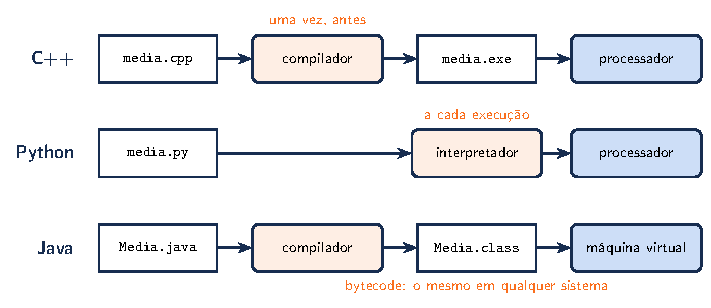
\includegraphics[width=0.9\linewidth,keepaspectratio]{imagens/capitulo-02_execucao.pdf}
\end{center}

Programas compilados costumam ser mais rápidos, porque toda a tradução foi feita antes, e o compilador encontra muitos erros sem que o programa precise rodar. Programas interpretados são mais práticos para testar ideias rapidamente, mas um erro só aparece quando a linha com problema é executada.

\subsubsection{As etapas da compilação em C++}

O que chamamos de ``compilar'' um programa em C++ são, na verdade, três etapas, executadas em sequência por um único comando:

\begin{center}
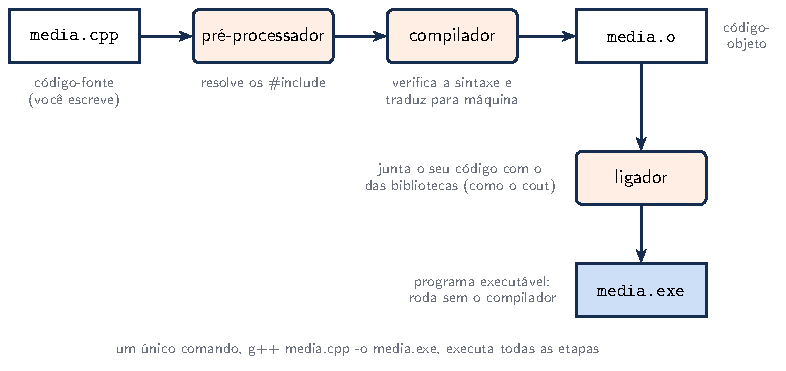
\includegraphics[width=0.9\linewidth,keepaspectratio]{imagens/capitulo-02_compilacao.pdf}
\end{center}

\begin{enumerate}
  \item O \textbf{pré-processador} trata as linhas que começam com \texttt{\#}, como o \texttt{\#include}, que copia para o programa as declarações de uma biblioteca.
  \item O \textbf{compilador} verifica a sintaxe e traduz o código para linguagem de máquina, gerando o \textbf{código-objeto}.
  \item O \textbf{ligador} (\textit{linker}) junta o código-objeto com o código das bibliotecas usadas, como a que implementa o \texttt{cout}, e gera o \textbf{executável}.
\end{enumerate}

\subsection{2.4 O ambiente de programação}

Para programar em C++, você precisa de duas coisas: um \textbf{editor}, onde escreve o código, e um \textbf{compilador}. O compilador mais usado é o \textbf{g++}, do projeto GCC, gratuito e disponível para Windows, Linux e macOS. No Windows, ele é instalado por pacotes como o MinGW-w64.

Uma \textbf{IDE} (ambiente de desenvolvimento integrado) reúne editor, compilador e depurador em um só programa, e permite compilar e executar com um clique. Algumas opções gratuitas: VS Code (com a extensão de C++), Code::Blocks e Dev-C++. Também existem compiladores on-line, que funcionam no navegador sem instalar nada, úteis para os primeiros exercícios.

Mesmo usando uma IDE, vale saber compilar pelo terminal, porque é isso que ela faz por baixo:

\begin{codigo}
\begin{Verbatim}[breaklines=true, breaksymbolleft={}, fontsize=\footnotesize]
$ g++ -Wall -Wextra media.cpp -o media
$ ./media
Digite a nota 1: 7
Digite a nota 2: 8
Aprovado! Média: 7.5
\end{Verbatim}
\end{codigo}

O \texttt{\$} representa o terminal, e não deve ser digitado. A primeira linha compila \texttt{media.cpp} e gera o executável \texttt{media} (no Windows, \texttt{media.exe}). As opções \texttt{-Wall -Wextra} ligam os \textbf{avisos} do compilador, que apontam trechos suspeitos mesmo quando não são erros de sintaxe: use-as sempre. A segunda linha executa o programa.

\subsection{2.5 A estrutura de um programa em C++}

Este é o programa mais simples que faz alguma coisa visível, e cada linha dele vai aparecer em todos os programas da apostila:

\begin{codigo}
\begin{Verbatim}[breaklines=true, breaksymbolleft={}, fontsize=\footnotesize]
// Meu primeiro programa em C++
#include <iostream>      // biblioteca de entrada e saída
using namespace std;     // cout em vez de std::cout

int main() {             // o programa começa aqui
    cout << "Olá, mundo!" << endl;
    return 0;            // 0 indica que terminou sem erro
}
\end{Verbatim}
\end{codigo}

\begin{itemize}
  \item \texttt{//} inicia um \textbf{comentário}, que vai até o fim da linha e é ignorado pelo compilador. Comentários de várias linhas ficam entre \texttt{/*} e \texttt{*/}.
  \item \texttt{\#include <iostream>} inclui a biblioteca de entrada e saída, que traz o \texttt{cout} e o \texttt{cin}.
  \item \texttt{using namespace std;} evita ter de escrever \texttt{std::} antes de \texttt{cout}, \texttt{cin} e \texttt{endl}, que pertencem ao ``espaço de nomes'' padrão, o \texttt{std}.
  \item \texttt{int main()} é a \textbf{função principal}: todo programa em C++ começa a ser executado por ela. O que está entre as chaves \texttt{\{ \}} é o \textbf{corpo} da função.
  \item Cada \textbf{instrução} termina com ponto e vírgula. Ele é para o C++ o que o ponto final é para uma frase.
  \item \texttt{return 0;} encerra o \texttt{main} e informa ao sistema que o programa terminou normalmente.
\end{itemize}

Espaços, linhas em branco e recuos não mudam o significado do programa, mas fazem enorme diferença para quem lê. O padrão desta apostila é recuar quatro espaços tudo o que está dentro de um par de chaves.

\subsection{2.6 Saída de dados com cout}

O \texttt{cout} (\textit{console output}) mostra dados na tela. O operador \texttt{<<} envia cada valor para ele, e vários valores podem ser encadeados em uma mesma instrução. O \texttt{endl} termina a linha; o caractere especial \texttt{\textbackslash n} faz o mesmo dentro de um texto.

\begin{codigo}
\begin{Verbatim}[breaklines=true, breaksymbolleft={}, fontsize=\footnotesize]
#include <iostream>
#include <iomanip>     // fixed e setprecision
using namespace std;

int main() {
    cout << "Linha 1" << endl;
    cout << "Linha 2\n";                  // \n também quebra
    cout << "Nome:\tAna\n";               // \t: tabulação
    cout << "Ela disse \"oi\"" << endl;   // \" : aspas no texto
    cout << "C:\\Arquivos" << endl;       // \\ : a própria barra
    cout << 7 << " + " << 3 << " = " << 7 + 3 << endl;
    // 7 + 3 = 10

    double preco = 55;
    cout << preco << endl;                           // 55
    cout << fixed << setprecision(2) << preco << endl;   // 55.00
    cout << 10.0 / 3 << endl;                        // 3.33
    return 0;
}
\end{Verbatim}
\end{codigo}

As combinações que começam com a barra invertida são as \textbf{sequências de escape}: elas representam caracteres que não daria para escrever diretamente no meio do texto. Para valores com casas decimais, \texttt{fixed} junto com \texttt{setprecision(2)}, da biblioteca \texttt{<iomanip>}, mostra sempre duas casas, o formato certo para dinheiro. Essa configuração continua valendo para todos os números mostrados depois dela, como o \texttt{3.33} da última linha.

No Portugol do VisuAlg, a mesma formatação é feita com dois números depois do valor: \texttt{escreval(preco:6:2)} mostra o preço com 6 posições no total e 2 casas decimais.

\subsection{2.7 Entrada de dados com cin}

O \texttt{cin} (\textit{console input}) lê dados digitados no teclado. O operador \texttt{>>} pega o próximo valor e o guarda na variável, convertendo-o para o tipo dela. Vários valores podem ser lidos de uma vez, separados por espaços ou por Enter.

O \texttt{>>} para de ler no primeiro espaço, então não serve para textos com espaços, como um nome completo. Para esses, use \texttt{getline}, que lê a linha inteira. Antes dele, \texttt{cin >> ws} descarta o Enter que o \texttt{>>} anterior deixou para trás; sem isso, o \texttt{getline} leria uma linha vazia.

\begin{codigo}
\begin{Verbatim}[breaklines=true, breaksymbolleft={}, fontsize=\footnotesize]
#include <iostream>
#include <string>
using namespace std;

int main() {
    int idade;
    double altura;
    cout << "Idade e altura: ";
    cin >> idade >> altura;        // ex.: 19 1.72
    string nome;
    cout << "Nome completo: ";
    cin >> ws;                     // descarta o Enter que sobrou
    getline(cin, nome);            // ex.: Ana Lima
    cout << nome << ", " << idade << " anos, " << altura << " m"
         << endl;                  // Ana Lima, 19 anos, 1.72 m
    return 0;
}
\end{Verbatim}
\end{codigo}

A variável \texttt{nome} é do tipo \texttt{string}, que guarda textos e precisa da biblioteca \texttt{<string>}. Os tipos de dados são o assunto do Capítulo 3, e os textos, do Capítulo 8.

\subsection{2.8 Um programa completo}

Com entrada, processamento e saída, já é possível transformar em programa o algoritmo da conta do restaurante, do Capítulo 1. Compare com o Portugol:

\begin{codigo}
\begin{Verbatim}[breaklines=true, breaksymbolleft={}, fontsize=\footnotesize]
algoritmo "DividirConta"
var
   conta, total, porPessoa: real
   pessoas: inteiro
inicio
   escreva("Valor da conta: ")
   leia(conta)
   escreva("Número de pessoas: ")
   leia(pessoas)
   total <- conta * 1.10
   porPessoa <- total / pessoas
   escreval("Total com serviço: R$ ", total:8:2)
   escreval("Cada pessoa paga: R$ ", porPessoa:8:2)
fimalgoritmo
\end{Verbatim}
\end{codigo}

\begin{codigo}
\begin{Verbatim}[breaklines=true, breaksymbolleft={}, fontsize=\footnotesize]
#include <iostream>
#include <iomanip>
using namespace std;

int main() {
    double conta, total, porPessoa;
    int pessoas;
    cout << "Valor da conta: ";
    cin >> conta;
    cout << "Número de pessoas: ";
    cin >> pessoas;
    total = conta * 1.10;               // 10% de serviço
    porPessoa = total / pessoas;
    cout << fixed << setprecision(2);
    cout << "Total com serviço: R$ " << total << endl;
    cout << "Cada pessoa paga: R$ " << porPessoa << endl;
    return 0;
}
// Exemplo de execução:
// Valor da conta: 200
// Número de pessoas: 4
// Total com serviço: R$ 220.00
// Cada pessoa paga: R$ 55.00
\end{Verbatim}
\end{codigo}

O resultado confere com o exemplo resolvido à mão no Capítulo 1: R\$ 55 por pessoa. Repare que \texttt{total / pessoas} divide um \texttt{double} por um \texttt{int}; como um dos lados tem casas decimais, o resultado também tem, e não há a surpresa da divisão inteira da Seção 2.2.

\subsection{2.9 Lendo as mensagens de erro}

Errar faz parte de programar, e o compilador é um aliado: ele aponta onde está o problema. Considere este programa, em que falta o ponto e vírgula no fim do \texttt{cout}:

\begin{codigo}
\begin{Verbatim}[breaklines=true, breaksymbolleft={}, fontsize=\footnotesize]
// erro de compilação: falta o ; no fim do cout
#include <iostream>
using namespace std;

int main() {
    cout << "Ola" << endl
    return 0;
}
\end{Verbatim}
\end{codigo}

O g++ responde:

\begin{codigo}
\begin{Verbatim}[breaklines=true, breaksymbolleft={}, fontsize=\footnotesize]
erro.cpp: In function 'int main()':
erro.cpp:6:26: error: expected ';' before 'return'
    6 |     cout << "Ola" << endl
      |                          ^
      |                          ;
\end{Verbatim}
\end{codigo}

A mensagem diz o arquivo (\texttt{erro.cpp}), a linha (6) e a coluna (26) do problema, o que ele esperava (``expected \texttt{\textquotesingle{};\textquotesingle{}}'', um ponto e vírgula) e ainda desenha onde ele deveria estar. Três dicas valem para qualquer mensagem:

\begin{itemize}
  \item \textbf{Comece pelo primeiro erro.} Um único erro pode causar uma cascata de mensagens seguintes; corrigido o primeiro, muitas delas desaparecem.
  \item \textbf{Olhe também a linha anterior.} O compilador percebe a falta do ponto e vírgula só quando encontra o \texttt{return}, na linha seguinte.
  \item \textbf{Leia a sugestão.} Ao usar uma variável \texttt{idad} que não existe, o g++ responde \texttt{\textquotesingle{}idad\textquotesingle{} was not declared in this scope; did you mean \textquotesingle{}idade\textquotesingle{}?}: ``\texttt{idad} não foi declarada; você quis dizer \texttt{idade}?''.
\end{itemize}

Além dos \textbf{erros}, que impedem a compilação, o compilador mostra \textbf{avisos} (\textit{warnings}), que não impedem, mas indicam algo suspeito, como uma variável declarada e nunca usada. Trate todo aviso como um erro a corrigir.

Os erros que o compilador encontra são os de \textbf{compilação}. Há ainda os erros de \textbf{execução}, quando o programa compila mas para no meio, por exemplo ao dividir um inteiro por zero, e os erros de \textbf{lógica}, quando ele roda até o fim mas dá a resposta errada. Esses dois últimos só aparecem testando, e é por isso que o teste de mesa do Capítulo 1 continua valendo depois que o programa existe.

\subsection{Erros Comuns}

\begin{itemize}
  \item \textbf{Esquecer o ponto e vírgula.} Toda instrução termina com \texttt{;}. Repare que a mensagem de erro costuma apontar para a linha seguinte.
  \item \textbf{Esquecer o \texttt{\#include}.} Sem \texttt{<iostream>}, o \texttt{cout} não existe; sem \texttt{<string>} ou \texttt{<iomanip>}, \texttt{string} e \texttt{setprecision} também não.
  \item \textbf{Trocar maiúsculas por minúsculas.} \texttt{Cout}, \texttt{Main} e \texttt{Int} não existem. O C++ diferencia as duas.
  \item \textbf{Inverter os operadores do cin e do cout.} Saída usa \texttt{<<} (os dados vão para o \texttt{cout}); entrada usa \texttt{>>} (os dados vêm do \texttt{cin} para a variável).
  \item \textbf{Ler um texto com espaços usando \texttt{>>}.} Só a primeira palavra é lida. Use \texttt{getline}, precedido de \texttt{cin >> ws} se houver uma leitura com \texttt{>>} antes.
  \item \textbf{Dividir inteiros esperando casas decimais.} \texttt{7 / 2} vale 3. Use pelo menos um valor com ponto decimal, como \texttt{7 / 2.0}.
  \item \textbf{Usar vírgula decimal.} Em C++, assim como no Portugol, \texttt{1,10} não é um número: escreva \texttt{1.10}.
  \item \textbf{Ignorar os avisos.} Compile sempre com \texttt{-Wall -Wextra} e leia o que o compilador diz.
\end{itemize}
